
%(BEGIN_QUESTION)
% Copyright 2007, Tony R. Kuphaldt, released under the Creative Commons Attribution License (v 1.0)
% This means you may do almost anything with this work of mine, so long as you give me proper credit

This is a simple rate-of-change detector circuit, designed to produce an alarm if the input signal rate-of-change becomes excessive:

$$\includegraphics[width=15.5cm]{i03616x01.eps}$$

Unfortunately, though, this circuit has a problem.  The alarm light always stays on, even when the pressure is known to be steady.  Your first diagnostic measurement is DC voltage between TP2 and TP7: there you measure a steady value of 2.39 volts.  Your next diagnostic measurement is between TP4 and TP7: there you measure 23.1 volts.

Identify the likelihood of each specified fault for this circuit.  Consider each fault one at a time (i.e. no coincidental faults), determining whether or not each fault could independently account for {\it all} measurements and symptoms in this circuit.

% No blank lines allowed between lines of an \halign structure!
% I use comments (%) instead, so that TeX doesn't choke.

$$\vbox{\offinterlineskip
\halign{\strut
\vrule \quad\hfil # \ \hfil & 
\vrule \quad\hfil # \ \hfil & 
\vrule \quad\hfil # \ \hfil \vrule \cr
\noalign{\hrule}
%
% First row
{\bf Fault} & {\bf Possible} & {\bf Impossible} \cr
%
\noalign{\hrule}
%
% Another row
$C_1$ failed open &  &  \cr
%
\noalign{\hrule}
%
% Another row
$R_1$ failed open &  &  \cr
%
\noalign{\hrule}
%
% Another row
$R_3$ failed open &  &  \cr
%
\noalign{\hrule}
%
% Another row
$R_4$ failed open &  &  \cr
%
\noalign{\hrule}
%
% Another row
$C_1$ failed shorted &  &  \cr
%
\noalign{\hrule}
%
% Another row
$R_1$ failed shorted &  &  \cr
%
\noalign{\hrule}
%
% Another row
$R_3$ failed shorted &  &  \cr
%
\noalign{\hrule}
%
% Another row
$R_4$ failed shorted &  &  \cr
%
\noalign{\hrule}
%
% Another row
$RLY_1$ coil failed open &  &  \cr
%
\noalign{\hrule}
%
% Another row
$U_1$ output failed to low supply rail &  &  \cr
%
\noalign{\hrule}
%
% Another row
$U_1$ output failed to high supply rail &  &  \cr
%
\noalign{\hrule}
} % End of \halign 
}$$ % End of \vbox

Finally, identify the {\it next} diagnostic test or measurement you would make on this system.  Explain how the result(s) of this next test or measurement help further identify the location and/or nature of the fault.

\vskip 20pt \vbox{\hrule \hbox{\strut \vrule{} {\bf Suggestions for Socratic discussion} \vrule} \hrule}

\begin{itemize}
\item{} Identify the effects of resistor $R_1$ failing open.
\item{} Identify the effects of resistor $R_3$ failing open.
\item{} Identify the effects of resistor $R_4$ failing open.
\item{} Identify the effects of the relay coil failing open.
\item{} Explain how electrical ``noise'' in the transmitter's signal could cause false alarms.
\end{itemize}

\underbar{file i01868}
%(END_QUESTION)





%(BEGIN_ANSWER)

% No blank lines allowed between lines of an \halign structure!
% I use comments (%) instead, so that TeX doesn't choke.

$$\vbox{\offinterlineskip
\halign{\strut
\vrule \quad\hfil # \ \hfil & 
\vrule \quad\hfil # \ \hfil & 
\vrule \quad\hfil # \ \hfil \vrule \cr
\noalign{\hrule}
%
% First row
{\bf Fault} & {\bf Possible} & {\bf Impossible} \cr
%
\noalign{\hrule}
%
% Another row
$C_1$ failed open &  & $\surd$ \cr
%
\noalign{\hrule}
%
% Another row
$R_1$ failed open & $\surd$ &  \cr
%
\noalign{\hrule}
%
% Another row
$R_3$ failed open &  & $\surd$ \cr
%
\noalign{\hrule}
%
% Another row
$R_4$ failed open & $\surd$ &  \cr
%
\noalign{\hrule}
%
% Another row
$C_1$ failed shorted & $\surd$ &  \cr
%
\noalign{\hrule}
%
% Another row
$R_1$ failed shorted &  & $\surd$ \cr
%
\noalign{\hrule}
%
% Another row
$R_3$ failed shorted &  & $\surd$ \cr
%
\noalign{\hrule}
%
% Another row
$R_4$ failed shorted &  & $\surd$ \cr
%
\noalign{\hrule}
%
% Another row
$RLY_1$ coil failed open &  & $\surd$ \cr
%
\noalign{\hrule}
%
% Another row
$U_1$ output failed to low supply rail &  & $\surd$ \cr
%
\noalign{\hrule}
%
% Another row
$U_1$ output failed to high supply rail & $\surd$ &  \cr
%
\noalign{\hrule}
} % End of \halign 
}$$ % End of \vbox

%(END_ANSWER)





%(BEGIN_NOTES)

A good ``next step'' would be to measure the DC voltage signals at both inputs of the opamp (TP3 and TP6), to see whether or not it is ``being told'' to energize the relay.  If so, the problem must lie before the opamp.  If not, the problem {\it is} the opamp.

%INDEX% Troubleshooting review: electric circuits

%(END_NOTES)


